\documentclass[pdflatex,sn-mathphys-num]{sn-jnl}

\usepackage{bookmark}
\usepackage{tabularx}
\usepackage{tikz}
\usetikzlibrary{shapes.geometric, shapes.misc, arrows.meta, positioning, calc}
\usepackage{graphicx}
\usepackage{multirow}
\usepackage{amsmath,amssymb,amsfonts}
\usepackage{booktabs}

\raggedbottom

\renewcommand{\thefigure}{S\arabic{figure}}
\renewcommand{\thetable}{S\arabic{table}}

\begin{document}

\title[Supplementary material: Which acoustic shift costs a CQT--CNN the most]{Supplementary material: Which Acoustic Shift Costs a CQT--CNN the Most? A Per-Seed Factorized Evaluation on Isolated Piano Chords}

\author*[1]{\fnm{Cikal} \sur{Gemintang Seya}}\email{cikalgemintangseya1@gmail.com}
\author[1]{\fnm{Jasman} \sur{Pardede}}\email{jasman@itenas.ac.id}
\affil*[1]{\orgdiv{Informatics}, \orgname{Institut Teknologi Nasional Bandung}, \orgaddress{\street{Neglasari}, \city{Bandung}, \postcode{40124}, \state{West Java}, \country{Indonesia}}}

\maketitle

This supplement documents the MIDI recorder, the six recorded datasets, the ten training runs behind the main article, the construction of the eval-only overlays, and the per-checkpoint tables the main article states only in summary. Dataset identifiers match the main text: \texttt{training}, \texttt{thinkpad}, \texttt{vivo}, \texttt{flow}, \texttt{thinkpad-2}, \texttt{flow-2}.

\section{Provenance of every number}\label{sec:provenance}

Every accuracy in the main article comes from ten checkpoints: two training-set variants (\texttt{orig}, \texttt{clean}) $\times$ five seeds (42--46), trained under an explicit stratified 80/10/10 split. An earlier 7{,}184-clip \texttt{clean} run that collapsed on Yamaha is not in this report, and no seed of the ten repeats that collapse.

Dataset-level figures (recorder, clip statistics, mean CQT shift, envelope decomposition, overlay CQT examples) measure the recorded audio or the overlay banks and do not depend on a checkpoint. Training curves, seed-spread, overlay-tax, and in-domain overlay figures come from the ten retrains. The $k$-fold figure comes from the five-fold runs of each variant.

\section{Dataset generator}\label{sec:generator}

All six datasets were captured with the same web recorder. The browser talks to the keyboard over USB MIDI and to one microphone at a time. Fig.~\ref{fig:esm-app} is the session screen. Fig.~\ref{fig:esm-flow} is the capture loop. Because the label is the MIDI trigger rather than a human annotation after the fact, class identity is identical across acoustic conditions by construction, which is what makes the factor comparison in the main article a comparison of recordings rather than of labelling.

\begin{figure}[t]
\centering
\includegraphics[width=0.92\textwidth]{ESM_1.png}
\caption{Web recorder used for every dataset. USB MIDI drives the keyboard; the selected microphone writes a labeled clip.}
\label{fig:esm-app}
\end{figure}

\begin{figure}[t]
  \centering
  \resizebox{!}{0.70\textheight}{%
  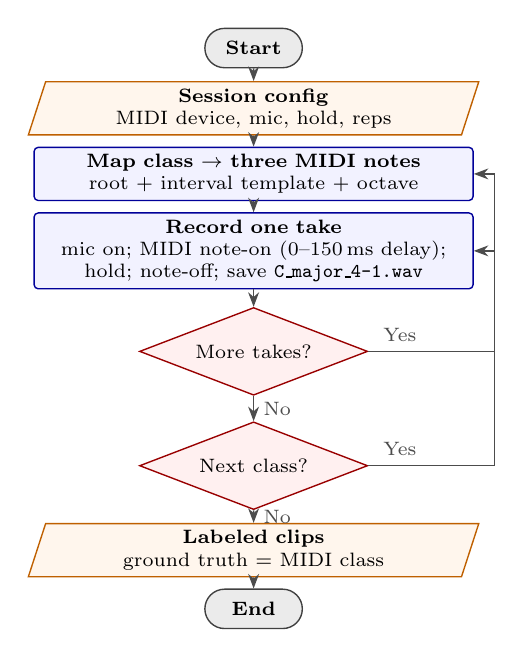
\begin{tikzpicture}[
    node distance=0.11cm and 0.10cm,
    >={Stealth},
    font=\scriptsize,
    base/.style={draw, align=center, minimum height=0.42cm, line width=0.5pt, inner sep=2.5pt},
    terminal/.style={base, shape=rounded rectangle, rounded rectangle arc length=180, draw=black!75, fill=black!8, minimum height=0.50cm, minimum width=1.8cm, inner xsep=8pt, font=\scriptsize\bfseries},
    process/.style={base, rectangle, rounded corners=1.5pt, draw=blue!60!black, fill=blue!5, text width=5.4cm},
    io/.style={base, trapezium, trapezium left angle=72, trapezium right angle=108, trapezium stretches body=true, draw=orange!75!black, fill=orange!7, text width=5.0cm, inner xsep=4pt},
    decision/.style={base, diamond, aspect=2.6, draw=red!60!black, fill=red!6, text width=2.2cm, inner sep=1pt},
    arrow/.style={->, line width=0.5pt, black!70}
  ]
    \node[terminal] (start) {Start};
    \node[io, below=0.16cm of start] (cfg)
    {\textbf{Session config}\\
     MIDI device, mic, hold, reps};
    \node[process, below=0.14cm of cfg] (map)
    {\textbf{Map class $\to$ three MIDI notes}\\
     root $+$ interval template $+$ octave};
    \node[process, below=0.14cm of map] (rec)
    {\textbf{Record one take}\\
     mic on; MIDI note-on (0--150\,ms delay);\\
     hold; note-off; save \texttt{C\_major\_4-1.wav}};
    \node[decision, below=0.22cm of rec] (morep)
    {More takes?};
    \node[decision, below=0.32cm of morep] (morec)
    {Next class?};
    \node[io, below=0.16cm of morec] (doneio)
    {\textbf{Labeled clips}\\
     ground truth $=$ MIDI class};
    \node[terminal, below=0.14cm of doneio] (endn) {End};
    \draw[arrow] (start) -- (cfg);
    \draw[arrow] (cfg) -- (map);
    \draw[arrow] (map) -- (rec);
    \draw[arrow] (rec) -- (morep);
    \draw[arrow] (morep.east) -- ++(1.6,0) node[above, font=\scriptsize, pos=0.25] {Yes}
      |- (rec.east);
    \draw[arrow] (morep) -- (morec) node[midway, right, font=\scriptsize] {No};
    \draw[arrow] (morec.east) -- ++(1.6,0) node[above, font=\scriptsize, pos=0.25] {Yes}
      |- (map.east);
    \draw[arrow] (morec) -- (doneio) node[midway, right, font=\scriptsize] {No};
    \draw[arrow] (doneio) -- (endn);
  \end{tikzpicture}%
  }
  \caption{Recorder loop. Class identity comes from the MIDI trigger, not from a human label after the fact.}
  \label{fig:esm-flow}
\end{figure}

Table~\ref{tab:esm-session} lists the session settings shared by every dataset.

\begin{table}[t]
\caption{Recorder session settings.}\label{tab:esm-session}
\begin{tabular}{@{}ll@{}}
\toprule
Parameter & Value \\
\midrule
Trigger & USB MIDI note-on (three notes) \\
Vocabulary & 12 roots $\times$ maj / min / dim, fourth octave \\
Voice & Grand-piano preset \\
Attack delay & 0--150\,ms (training) \\
Sample rate & 48{,}000\,Hz, mono \\
Training format & OGG/OPUS, 32-bit \\
Eval format & WAV \\
CQT window & first 2.0\,s of each clip \\
\bottomrule
\end{tabular}
\end{table}

\section{Dataset characteristics}\label{sec:datasets}

Table~\ref{tab:esm-inventory} is the inventory. Every dataset has all 36 classes and a constant take count (200 or 40). No class folder is missing. Durations sit above the 2.0\,s CQT crop. ThinkPad recordings are quieter than Vivo and Flow. Training CQT centroids sit higher ($\approx$467\,Hz) than the held-out sets ($\approx$269--323\,Hz).

Sixteen training clips are digital silence (peak $=0$), all of them $C$ diminished, which is 8\% of that class. Twelve further $A\sharp$ major takes are exact CQT duplicates of another take of the same class. \texttt{clean} drops the sixteen silent clips and one member of each duplicate pair (7{,}172 remaining). Vivo has 489 near-clip takes (hotter phone mic). No dataset has hard clipping.

\begin{table}[t]
\caption{Recorded datasets. Per-class count is constant. Duration and RMS are over all takes.}\label{tab:esm-inventory}
\setlength{\tabcolsep}{3.2pt}
\begin{tabular}{@{}llrrrrrr@{}}
\toprule
Dataset & Fmt & $N$ & /cls & Dur.\ min & Dur.\ mean & RMS dB & Cent.\ Hz \\
\midrule
\texttt{training} & OGG & 7{,}200 & 200 & 2.00 & 2.40 & $-21.4$ & 467 \\
\texttt{thinkpad} & WAV & 1{,}440 & 40 & 2.10 & 2.45 & $-26.6$ & 323 \\
\texttt{vivo} & WAV & 1{,}440 & 40 & 2.10 & 2.44 & $-19.2$ & 290 \\
\texttt{flow} & WAV & 1{,}440 & 40 & 2.10 & 2.44 & $-19.6$ & 269 \\
\texttt{thinkpad-2} & WAV & 1{,}440 & 40 & 2.16 & 2.52 & $-26.8$ & 310 \\
\texttt{flow-2} & WAV & 1{,}440 & 40 & 2.16 & 2.44 & $-22.6$ & 313 \\
\bottomrule
\end{tabular}
\end{table}

Fig.~\ref{fig:esm-chars} shows the same three quantities as distributions. Duration spread on \texttt{training} is the 0--150\,ms attack delay. The \texttt{thinkpad-2} tail above 3\,s is a longer hold, not a missing class. RMS separates the ThinkPad microphone from Vivo and Flow. Centroid separates the training tablet from every held-out microphone.

\begin{figure}[t]
\centering
\includegraphics[width=\textwidth]{esm-dataset-chars.pdf}
\caption{Dataset characteristics.
\textbf{(A)}~clip duration;
\textbf{(B)}~waveform RMS (training silence at $-240$\,dB clipped to $-40$ for display);
\textbf{(C)}~CQT spectral centroid.}
\label{fig:esm-chars}
\end{figure}

Fig.~\ref{fig:esm-cqt} is the mean CQT of each held-out dataset minus the training mean. Recording-setting datasets are cooler in the mid bins and hotter at the bottom. The two Yamaha datasets share a low-bin excess that the Techno recording-setting datasets do not, which is the keyboard factor visible in the feature the network reads.

\begin{figure}[t]
\centering
\includegraphics[width=\textwidth]{esm-cqt-shift.pdf}
\caption{Mean CQT difference: held-out mean minus training mean (dB). Same color scale on every panel.}
\label{fig:esm-cqt}
\end{figure}

\subsection{How much of the shift is a per-clip envelope offset}\label{sec:envelope}

Fig.~\ref{fig:esm-envelope} measures the shift in the two quantities a per-clip normalization would remove. Panel A is each clip's own dB mean over its $216\times188$ CQT. The held-out datasets sit between 8\,dB below (\texttt{vivo}, $-60.3$) and 7\,dB above (\texttt{thinkpad-2}, $-44.7$) the training mean of $-51.9$\,dB, so a large part of what changes with microphone or keyboard is a global level, not a change of shape.

Panel B decomposes each class centroid's drift from its training centroid into an offset component (what mean-centering removes), a scale component (what unit-normalizing removes), and a residual. Averaged over the 36 classes, the offset and scale terms together account for 31\% of the drift on \texttt{thinkpad}, 30\% on \texttt{flow}, 47\% on \texttt{flow-2}, 54\% on \texttt{thinkpad-2}, and 56\% on \texttt{vivo}. The residual is the larger share on three of five datasets, so the shift is not purely a level change; but the offset and scale components are exactly what the network's frequency-axis batch normalization fixes once to the training distribution and then cannot adapt at inference, which is the mechanism the main article infers from the error structure.

\begin{figure}[t]
\centering
\includegraphics[width=\textwidth]{esm-envelope-shift.pdf}
\caption{Envelope shift.
\textbf{(A)}~per-clip mean CQT level;
\textbf{(B)}~share of each class centroid's drift from training explained by a per-clip offset, a per-clip scale, and the residual.}
\label{fig:esm-envelope}
\end{figure}

\section{Training protocol and per-checkpoint record}\label{sec:training}

Every run was launched as its own operating-system process with \texttt{TF\_DETERMINISTIC\_OPS=1} and batch size 32, so no two runs share a CUDA context and the spread reported below is not kernel-selection noise across devices. The seed sets an explicit stratified 80/10/10 split (a 10\% test hold-out, then a stratified $1/9$ of the remainder as validation), the weight initialization, and the Python, NumPy, and TensorFlow global generators. Fit uses that validation partition as \texttt{validation\_data}, not Keras \texttt{validation\_split}. Split membership is written to disk for every run.

Table~\ref{tab:esm-checkpoints} is the training record of all ten checkpoints. \texttt{EarlyStopping} has patience 6 and restores the best-validation-loss weights, so the restored epoch is always six less than the epochs run. Every run reaches 1.000 accuracy on its own held-out Techno test split (720 clips on \texttt{orig}, 718 on \texttt{clean}).

\begin{table}[t]
\caption{Per-checkpoint training record. \emph{Restored} is the epoch whose weights early stopping kept. In-domain accuracy is on each run's own held-out 10\% split.}\label{tab:esm-checkpoints}
\setlength{\tabcolsep}{3.2pt}
\begin{tabular}{@{}llrrrrrrr@{}}
\toprule
Variant & Seed & $N_{\text{train}}$ & $N_{\text{val}}$ & $N_{\text{test}}$ & Ep. & Rest. & Acc. & F1 \\
\midrule
\texttt{orig} & 42 & 5{,}760 & 720 & 720 & 16 & 10 & 1.0000 & 1.0000 \\
\texttt{orig} & 43 & 5{,}760 & 720 & 720 & 14 & 8 & 1.0000 & 1.0000 \\
\texttt{orig} & 44 & 5{,}760 & 720 & 720 & 24 & 18 & 1.0000 & 1.0000 \\
\texttt{orig} & 45 & 5{,}760 & 720 & 720 & 9 & 3 & 1.0000 & 1.0000 \\
\texttt{orig} & 46 & 5{,}760 & 720 & 720 & 21 & 15 & 1.0000 & 1.0000 \\
\texttt{clean} & 42 & 5{,}736 & 718 & 718 & 12 & 6 & 1.0000 & 1.0000 \\
\texttt{clean} & 43 & 5{,}736 & 718 & 718 & 33 & 27 & 1.0000 & 1.0000 \\
\texttt{clean} & 44 & 5{,}736 & 718 & 718 & 9 & 3 & 1.0000 & 1.0000 \\
\texttt{clean} & 45 & 5{,}736 & 718 & 718 & 20 & 14 & 1.0000 & 1.0000 \\
\texttt{clean} & 46 & 5{,}736 & 718 & 718 & 14 & 8 & 1.0000 & 1.0000 \\
\bottomrule
\end{tabular}
\end{table}

Fig.~\ref{fig:esm-history} shows the validation curves of the ten reported runs. Every run reaches 1.000 validation accuracy by epoch 2, so panel A separates nothing. Panel B does separate the runs, but not usefully: best validation loss ranges over six orders of magnitude, from $1.5\times10^{-9}$ to $2.2\times10^{-3}$, and its correlation with mean out-of-domain accuracy across the ten checkpoints is $-0.16$ (Pearson on $\log_{10}$ loss; Spearman $-0.28$). The restored epoch correlates at $r=0.04$. The run with the worst validation loss is \texttt{clean} seed 44, which is the strongest out-of-domain checkpoint in the study (mean recorded accuracy 0.981). The weakest out-of-domain checkpoint is \texttt{clean} seed 42 (mean 0.782). No quantity available at model-selection time predicts which checkpoint will transfer.

\begin{figure}[t]
\centering
\includegraphics[width=\textwidth]{esm-variant-history.pdf}
\caption{Validation curves of the ten reported checkpoints.
\textbf{(A)}~validation accuracy;
\textbf{(B)}~validation loss, log scale. The heavy line is \texttt{clean} seed 44, the worst validation loss and the strongest out-of-domain run.}
\label{fig:esm-history}
\end{figure}

Table~\ref{tab:esm-kfold} and Fig.~\ref{fig:esm-kfold} are the five-fold in-domain cross-validation of Scenario~1. An outer stratified fold holds out 20\% as test; a stratified $1/8$ of the remainder is validation, so each fold is 70/10/20 of the pool. Each fold is retrained from a fresh initialization. Mean test accuracy is 0.9999 on both variants. Two folds miss a single clip: \texttt{orig} fold 1 (0.9993 of 1{,}440) and \texttt{clean} fold 3 (0.9993 of 1{,}434). The axis in Fig.~\ref{fig:esm-kfold} is zoomed so those two misses are visible.

\begin{table}[t]
\caption{CNN in-domain 5-fold results. Each fold is 70/10/20 of the pool.}\label{tab:esm-kfold}
\setlength{\tabcolsep}{3.2pt}
\begin{tabular}{@{}llrrrrrr@{}}
\toprule
Variant & Fold & $N_{\text{train}}$ & $N_{\text{val}}$ & $N_{\text{test}}$ & Ep. & Acc. & F1 \\
\midrule
\texttt{orig} & 1 & 5{,}040 & 720 & 1{,}440 & 15 & 0.9993 & 0.9993 \\
\texttt{orig} & 2 & 5{,}040 & 720 & 1{,}440 & 14 & 1.0000 & 1.0000 \\
\texttt{orig} & 3 & 5{,}040 & 720 & 1{,}440 & 19 & 1.0000 & 1.0000 \\
\texttt{orig} & 4 & 5{,}040 & 720 & 1{,}440 & 20 & 1.0000 & 1.0000 \\
\texttt{orig} & 5 & 5{,}040 & 720 & 1{,}440 & 23 & 1.0000 & 1.0000 \\
\texttt{orig} & Mean & 5{,}040 & 720 & 1{,}440 & 18.2 & 0.9999 & 0.9999 \\
\texttt{clean} & 1 & 5{,}019 & 718 & 1{,}435 & 11 & 1.0000 & 1.0000 \\
\texttt{clean} & 2 & 5{,}019 & 718 & 1{,}435 & 18 & 1.0000 & 1.0000 \\
\texttt{clean} & 3 & 5{,}020 & 718 & 1{,}434 & 28 & 0.9993 & 0.9993 \\
\texttt{clean} & 4 & 5{,}020 & 718 & 1{,}434 & 20 & 1.0000 & 1.0000 \\
\texttt{clean} & 5 & 5{,}020 & 718 & 1{,}434 & 11 & 1.0000 & 1.0000 \\
\texttt{clean} & Mean & 5{,}020 & 718 & 1{,}434 & 17.6 & 0.9999 & 0.9999 \\
\bottomrule
\end{tabular}
\end{table}

\begin{figure}[t]
\centering
\includegraphics[width=\textwidth]{esm-cnn-kfold.pdf}
\caption{Five-fold in-domain test accuracy. The axis is zoomed to the range 0.9986--1.0003 so the two one-clip misses (\texttt{orig} fold 1, \texttt{clean} fold 3) are visible.}
\label{fig:esm-kfold}
\end{figure}

\section{Recorded out-of-domain results, per checkpoint}\label{sec:recorded}

Fig.~\ref{fig:esm-seed-spread} places all ten checkpoints on the five recorded held-out datasets. The vertical extent of each cluster, not its mean, is the object of the main article: on \texttt{thinkpad-2} the ten checkpoints run from 0.689 to 0.955, and on \texttt{vivo} from 0.670 to 0.994. No cell falls to the 0.348 Yamaha collapse of the earlier 7{,}184-clip \texttt{clean} run.

\begin{figure}[t]
\centering
\includegraphics[width=\textwidth]{esm-seed-spread-cnn.pdf}
\caption{Accuracy of every reported checkpoint on the five recorded held-out datasets. Dashes are per-variant means.}
\label{fig:esm-seed-spread}
\end{figure}

Table~\ref{tab:esm-factors} expands the factor ranking of the main article into all twenty comparisons. The keyboard gap is the Techno accuracy minus the matched Yamaha accuracy on the same checkpoint and recording setting; the recording-setting cost is $1.000$ minus that same Techno accuracy. The gap is positive on 19 of 20 rows. The remaining cell, \texttt{clean} seed 43 on Flow, is $-0.1$ points and sits inside the $\pm3$-point resolution. The gap exceeds the recording-setting cost on 17 of the 20 comparisons. All three exceptions fall on the Flow pair. One row has the two costs within 3 points of each other.

\begin{table}[t]
\caption{All twenty matched factor comparisons, in accuracy points. \emph{Gap} is the keyboard cost, \emph{RS} the recording-setting cost. $^\ast$Recording setting is the larger factor. $^\circ$The two costs differ by less than 3 points. $^\dagger$Gap inside the $\pm3$-point resolution.}\label{tab:esm-factors}
\setlength{\tabcolsep}{4pt}
\begin{tabular}{@{}llrrrrl@{}}
\toprule
Variant & Seed & Pair & Techno & Yamaha & Gap & RS \\
\midrule
\texttt{orig} & 42 & ThinkPad & 0.995 & 0.858 & 13.7 & 0.5 \\
\texttt{orig} & 42 & Flow & 0.949 & 0.854 & 9.4 & 5.1 \\
\texttt{orig} & 43 & ThinkPad & 0.935 & 0.689 & 24.6 & 6.5 \\
\texttt{orig} & 43 & Flow & 0.836 & 0.721 & 11.5 & 16.4$^\ast$ \\
\texttt{orig} & 44 & ThinkPad & 0.972 & 0.778 & 19.3 & 2.8 \\
\texttt{orig} & 44 & Flow & 0.986 & 0.791 & 19.5 & 1.4 \\
\texttt{orig} & 45 & ThinkPad & 0.979 & 0.761 & 21.8 & 2.1 \\
\texttt{orig} & 45 & Flow & 0.998 & 0.772 & 22.6 & 0.2 \\
\texttt{orig} & 46 & ThinkPad & 0.995 & 0.907 & 8.8 & 0.5 \\
\texttt{orig} & 46 & Flow & 0.998 & 0.924 & 7.4 & 0.2 \\
\texttt{clean} & 42 & ThinkPad & 0.962 & 0.738 & 22.4 & 3.8 \\
\texttt{clean} & 42 & Flow & 0.829 & 0.711 & 11.8 & 17.1$^\ast$ \\
\texttt{clean} & 43 & ThinkPad & 0.960 & 0.878 & 8.3 & 4.0 \\
\texttt{clean} & 43 & Flow & 0.894 & 0.896 & $-0.1^\dagger$ & 10.6$^\ast$ \\
\texttt{clean} & 44 & ThinkPad & 1.000 & 0.955 & 4.5 & 0.0 \\
\texttt{clean} & 44 & Flow & 0.996 & 0.965 & 3.1 & 0.4$^\circ$ \\
\texttt{clean} & 45 & ThinkPad & 0.999 & 0.858 & 14.0 & 0.1 \\
\texttt{clean} & 45 & Flow & 0.982 & 0.882 & 10.0 & 1.8 \\
\texttt{clean} & 46 & ThinkPad & 0.999 & 0.895 & 10.3 & 0.1 \\
\texttt{clean} & 46 & Flow & 0.991 & 0.917 & 7.4 & 0.9 \\
\bottomrule
\end{tabular}
\end{table}

\section{Eval-only overlays}\label{sec:overlays}

\subsection{Bank construction}\label{sec:banks}

\emph{Noise.} 400 ESC-50 clips \cite{Piczak2015}, the complete interior and domestic group: \texttt{can\_opening}, \texttt{clock\_alarm}, \texttt{clock\_tick}, \texttt{door\_wood\_creaks}, \texttt{door\_wood\_knock}, \texttt{glass\_breaking}, \texttt{keyboard\_typing}, \texttt{mouse\_click}, \texttt{vacuum\_cleaner}, \texttt{washing\_machine}, 40 clips each. Each is reduced to a 2.0\,s segment of maximum energy and converted to a $216\times188$ CQT under the same hop and binning as the chord features. Mixing is in the CQT power domain, one noise matrix per chord clip at a broadband SNR drawn uniformly from $[10,25]$\,dB, with the noise matrix rolled in time by a random offset.

\emph{Room impulse responses.} The IR Survey \cite{Traer2016} contributes 174 responses spanning 51 indoor room types (bedrooms, classrooms, offices, kitchens, halls, galleries, and similar), after removing bathrooms, showers, outdoor and semi-outdoor spaces, and vehicles and transit stations. Responses are made mono, resampled to 48\,kHz, trimmed of leading silence below $-40$\,dB relative to peak, and peak-normalized. Durations run 0.18--1.99\,s, median 0.62\,s.

\emph{Microphone impulse responses.} 67 vintage-capsule device impulse responses from micIRP, the vintage half of the DIR set Kusaka and Maezawa use at train time \cite{Kusaka2024}, prepared identically to the room bank.

Both impulse-response banks convolve the evaluation waveform before CQT extraction, one response drawn per clip, with a fixed draw seed. Nothing is written back into training. The overlays hit the five held-out datasets and each checkpoint's Techno test split.

Fig.~\ref{fig:esm-overlay-cqt} shows one clip under each overlay in the CQT the network actually sees. Noise fills the gaps between partials, the room response smears energy across frames, and the microphone response darkens the low bins as a spectral tilt without adding a partial. That last panel is the visual form of the result in Section~\ref{sec:overlay-results}: a capsule response moves the level, not the interval structure.

\begin{figure}[t]
\centering
\includegraphics[width=\textwidth]{esm-overlay-cqt.pdf}
\caption{One \texttt{vivo} take of $C$ maj (top) and $E$ dim (bottom) after each eval-only overlay. These are the stored CQT matrices, not time-domain mixes.}
\label{fig:esm-overlay-cqt}
\end{figure}

\subsection{Per-checkpoint overlay results}\label{sec:overlay-results}

The main article gives every seed under noise and reports only means for the other two overlays. Tables~\ref{tab:esm-rir} and~\ref{tab:esm-dir} give the room and microphone responses per checkpoint, and Fig.~\ref{fig:esm-overlay-tax} plots all three taxes together.

\begin{table}[t]
\caption{Accuracy under eval-only indoor room impulse responses, per checkpoint.}\label{tab:esm-rir}
\setlength{\tabcolsep}{4pt}
\begin{tabular}{@{}llrrrrr@{}}
\toprule
Variant & Seed & \texttt{thinkpad} & \texttt{vivo} & \texttt{flow} & \texttt{thinkpad-2} & \texttt{flow-2} \\
\midrule
\texttt{orig} & 42 & 0.876 & 0.782 & 0.892 & 0.771 & 0.769 \\
\texttt{orig} & 43 & 0.841 & 0.687 & 0.810 & 0.553 & 0.579 \\
\texttt{orig} & 44 & 0.919 & 0.868 & 0.936 & 0.707 & 0.707 \\
\texttt{orig} & 45 & 0.931 & 0.893 & 0.962 & 0.736 & 0.753 \\
\texttt{orig} & 46 & 0.951 & 0.890 & 0.962 & 0.868 & 0.888 \\
\texttt{orig} & Mean & 0.903 & 0.824 & 0.913 & 0.727 & 0.739 \\
\texttt{clean} & 42 & 0.837 & 0.623 & 0.799 & 0.656 & 0.662 \\
\texttt{clean} & 43 & 0.865 & 0.739 & 0.872 & 0.772 & 0.778 \\
\texttt{clean} & 44 & 0.934 & 0.912 & 0.943 & 0.881 & 0.874 \\
\texttt{clean} & 45 & 0.922 & 0.837 & 0.920 & 0.772 & 0.776 \\
\texttt{clean} & 46 & 0.958 & 0.903 & 0.962 & 0.831 & 0.811 \\
\texttt{clean} & Mean & 0.903 & 0.803 & 0.899 & 0.782 & 0.780 \\
\bottomrule
\end{tabular}
\end{table}

\begin{table}[t]
\caption{Accuracy under eval-only 67-capsule microphone impulse responses, per checkpoint.}\label{tab:esm-dir}
\setlength{\tabcolsep}{4pt}
\begin{tabular}{@{}llrrrrr@{}}
\toprule
Variant & Seed & \texttt{thinkpad} & \texttt{vivo} & \texttt{flow} & \texttt{thinkpad-2} & \texttt{flow-2} \\
\midrule
\texttt{orig} & 42 & 0.978 & 0.870 & 0.929 & 0.840 & 0.838 \\
\texttt{orig} & 43 & 0.937 & 0.779 & 0.831 & 0.653 & 0.690 \\
\texttt{orig} & 44 & 0.973 & 0.938 & 0.957 & 0.735 & 0.773 \\
\texttt{orig} & 45 & 0.960 & 0.947 & 0.983 & 0.776 & 0.801 \\
\texttt{orig} & 46 & 0.990 & 0.943 & 0.990 & 0.904 & 0.910 \\
\texttt{orig} & Mean & 0.968 & 0.895 & 0.938 & 0.782 & 0.802 \\
\texttt{clean} & 42 & 0.938 & 0.705 & 0.797 & 0.738 & 0.723 \\
\texttt{clean} & 43 & 0.963 & 0.818 & 0.896 & 0.848 & 0.860 \\
\texttt{clean} & 44 & 0.991 & 0.982 & 0.973 & 0.943 & 0.950 \\
\texttt{clean} & 45 & 0.987 & 0.908 & 0.957 & 0.846 & 0.867 \\
\texttt{clean} & 46 & 0.992 & 0.983 & 0.975 & 0.865 & 0.883 \\
\texttt{clean} & Mean & 0.974 & 0.879 & 0.919 & 0.848 & 0.857 \\
\bottomrule
\end{tabular}
\end{table}

\begin{figure}[t]
\centering
\includegraphics[width=\textwidth]{esm-overlay-tax.pdf}
\caption{Overlay tax per checkpoint, recorded accuracy minus overlay accuracy.
\textbf{(A)}~ESC-50 interior noise;
\textbf{(B)}~indoor room impulse response;
\textbf{(C)}~67-capsule microphone impulse response. Dashes are per-variant means. Negative values are overlays that helped.}
\label{fig:esm-overlay-tax}
\end{figure}

Two features of Fig.~\ref{fig:esm-overlay-tax} are worth stating explicitly. First, the noise tax is larger on the two Yamaha datasets than on the three Techno ones under both variants: 17.4 and 16.4 points against 11.0, 10.2, and 9.8 on \texttt{orig}, and 11.1 and 11.2 against 8.5, 9.6, and 9.1 on \texttt{clean}. Keyboard shift plus noise is the worst condition in the study. Second, the 67-capsule microphone tax sits near zero, with means of 1.4 points on \texttt{orig} and 1.2 on \texttt{clean}. Averaged over the three Techno datasets it is 1.4 points on \texttt{orig} and 0.9 on \texttt{clean}, against 5.2--6.7 points for an actual change of microphone. Convolution with a vintage capsule response is not a substitute for recording through a different device.

Table~\ref{tab:esm-indomain} and Fig.~\ref{fig:esm-indomain} apply the same three overlays to each checkpoint's Techno test split, so the tax has no recorded device or keyboard change underneath it. Mean taxes are 6.9 / 2.2 / 0.9 points on \texttt{orig} and 4.3 / 1.7 / 0.4 on \texttt{clean} for noise, room, and DIR. DIR is cheap with no recorded device change, so the bank is a weak transform rather than a tax that only vanishes after a mic has already moved. Noise and room cost more once the recording is already shifted.

\begin{table}[t]
\caption{Accuracy on each checkpoint's Techno test split under eval-only overlays. The dry column is 1.000 for every seed.}\label{tab:esm-indomain}
\setlength{\tabcolsep}{4pt}
\begin{tabular}{@{}llrrrr@{}}
\toprule
Variant & Seed & $N$ & Noise & RIR & DIR \\
\midrule
\texttt{orig} & 42 & 720 & 0.912 & 0.968 & 0.990 \\
\texttt{orig} & 43 & 720 & 0.900 & 0.961 & 0.988 \\
\texttt{orig} & 44 & 720 & 0.906 & 0.989 & 0.997 \\
\texttt{orig} & 45 & 720 & 0.969 & 0.978 & 0.990 \\
\texttt{orig} & 46 & 720 & 0.969 & 0.996 & 0.992 \\
\texttt{orig} & Mean & 720 & 0.931 & 0.978 & 0.991 \\
\texttt{clean} & 42 & 718 & 0.944 & 0.961 & 0.997 \\
\texttt{clean} & 43 & 718 & 0.929 & 0.978 & 0.996 \\
\texttt{clean} & 44 & 718 & 0.981 & 0.992 & 0.993 \\
\texttt{clean} & 45 & 718 & 0.950 & 0.989 & 0.997 \\
\texttt{clean} & 46 & 718 & 0.982 & 0.996 & 0.994 \\
\texttt{clean} & Mean & 718 & 0.957 & 0.983 & 0.996 \\
\bottomrule
\end{tabular}
\end{table}

\begin{figure}[t]
\centering
\includegraphics[width=\textwidth]{esm-indomain-overlay.pdf}
\caption{Overlay tax on each checkpoint's Techno test split. Dashes are per-variant means.}
\label{fig:esm-indomain}
\end{figure}

\section{Where the error lands}\label{sec:perclass}

Table~\ref{tab:esm-quality} is per-quality recall averaged over the five seeds of each variant. Diminished triads, the closest-packed template, are the weakest quality on both Yamaha datasets under both variants, and are already the weakest on \texttt{vivo} under a recording-setting change alone.

\begin{table}[t]
\caption{Recall by chord quality, mean over the five seeds of each variant.}\label{tab:esm-quality}
\setlength{\tabcolsep}{5pt}
\begin{tabular}{@{}llrrr@{}}
\toprule
Variant & Dataset & Major & Minor & Dim \\
\midrule
\texttt{orig} & \texttt{thinkpad} & 0.986 & 0.975 & 0.964 \\
\texttt{orig} & \texttt{vivo} & 0.978 & 0.903 & 0.865 \\
\texttt{orig} & \texttt{flow} & 0.980 & 0.947 & 0.934 \\
\texttt{orig} & \texttt{thinkpad-2} & 0.844 & 0.808 & 0.745 \\
\texttt{orig} & \texttt{flow-2} & 0.838 & 0.831 & 0.768 \\
\texttt{clean} & \texttt{thinkpad} & 0.980 & 0.983 & 0.989 \\
\texttt{clean} & \texttt{vivo} & 0.910 & 0.907 & 0.812 \\
\texttt{clean} & \texttt{flow} & 0.937 & 0.954 & 0.924 \\
\texttt{clean} & \texttt{thinkpad-2} & 0.888 & 0.905 & 0.802 \\
\texttt{clean} & \texttt{flow-2} & 0.890 & 0.905 & 0.828 \\
\bottomrule
\end{tabular}
\end{table}

Which \emph{individual} classes fail is not stable across seeds, and this is the main correction the per-seed protocol makes to a single-run reading. Table~\ref{tab:esm-zero} counts, for each variant and dataset, how many of the 36 classes reach zero recall on at least one seed and how many (class, seed) cells that involves. On \texttt{orig}/\texttt{thinkpad-2}, eleven different classes hit zero on at least one of five seeds. Both Techno ThinkPad columns are empty: no class reaches zero recall there in any run. An earlier single checkpoint showed zero recall on $D$ minor, $E$ diminished, and $G\sharp$ diminished; across the ten reported checkpoints those three are unremarkable, and a per-class error story told from one run would have named the wrong classes.

\begin{table}[t]
\caption{Zero-recall incidence across the five seeds of each variant. \emph{Classes} is how many of the 36 reach zero recall on at least one seed; \emph{cells} is the number of (class, seed) pairs at zero.}\label{tab:esm-zero}
\setlength{\tabcolsep}{5pt}
\begin{tabular}{@{}lrrrr@{}}
\toprule
 & \multicolumn{2}{c}{\texttt{orig}} & \multicolumn{2}{c}{\texttt{clean}} \\
\cmidrule(lr){2-3} \cmidrule(lr){4-5}
Dataset & Classes & Cells & Classes & Cells \\
\midrule
\texttt{thinkpad} & 0 & 0 & 0 & 0 \\
\texttt{vivo} & 3 & 4 & 5 & 7 \\
\texttt{flow} & 2 & 2 & 3 & 4 \\
\texttt{thinkpad-2} & 11 & 15 & 6 & 7 \\
\texttt{flow-2} & 9 & 13 & 6 & 8 \\
\bottomrule
\end{tabular}
\end{table}

\subsection{The weakest cells}\label{sec:weakest}

The weakest recorded cells stay above 0.67. They belong to \texttt{clean} seed 42 on \texttt{vivo} (0.670) and \texttt{orig} seed 43 on the two Yamaha sets (0.689 / 0.721). \texttt{clean} seed 42 is also a weak Yamaha run (0.738 / 0.711), while the same seed under \texttt{orig} scores 0.858 / 0.854. The two runs do not share a data partition, so nothing here attributes the gap to the 28 dropped clips on their own. The strongest cells belong to \texttt{clean} seed 44 (Yamaha 0.955 / 0.965, \texttt{vivo} 0.990), the run with the worst validation loss (Section~\ref{sec:training}).

\section{Reproducibility}\label{sec:repro}

Software: Python 3.10, TensorFlow 2.15, scikit-learn 1.7.2, Librosa 0.11.0, NumPy 1.26.4, Matplotlib 3.10.8. Training ran with \texttt{TF\_DETERMINISTIC\_OPS=1}, one operating-system process per run. Feature extraction and evaluation used a ROG Flow X13 (Ryzen 7 6800HS, 16\,GB RAM) and Google Colaboratory (T4/A100).

CQT extraction is identical for training, every recorded dataset, and every overlay: \texttt{librosa.cqt()} at 48\,kHz, hop 512, Hann window, 6 octaves from C1 at 36 bins per octave, first 2.0\,s of each clip, magnitudes to dB with \texttt{amplitude\_to\_db(ref=max)}, stored as $216\times188\times1$.

The recorded datasets are at \url{https://zenodo.org/records/21077144} and the recording tool at \url{https://github.com/sglkc/chords-dataset-generator/}. The training record, per-epoch curves, recorded and overlay accuracies, Techno-test overlay taxes, and per-class recall of all ten checkpoints are reproducible from those datasets under the settings given in this section.

\bibliography{mendeley}

\end{document}
